\chapter{Interface}
\label{cha:interface}
\raggedbottom
\renewcommand\arraystretch{1.75}

%%% Local Variables: 
%%% mode: latex
%%% TeX-master: ug.tex
%%% End: 



\section{Basic Ideas of the Interface}

The basic idea of the ScaFaCoS interface is that it should be very simple to include the library to existing programs and packages.
Therefore the aim was to have as few required functions as possible for adding the library. To use the library one has only five functions
to add to an existing code, if the default parameters for each solver suffice. Of course there is the possibility to change the
parameters of the solvers by use of additional functions. In this sections the basic functions will be described, so that the reader
is able to add the ScaFaCoS library to his or her own code. \\
To understand the following sections, one has to know the idea behind the use of the library. One usage cycle is divided into five
sections, which are mapped to the five required functions. These sections are:
\begin{enumerate}
  \item Initialization of the library
  \item Setting the non-solver specific parameters
  \item Tuning the solver
  \item Running the solver (more then once if needed)
  \item Destroying allocated resources of the library
\end{enumerate}
These five steps are each tied to one call of the respective function. In the initialization step the communicator used by the library is
defined, as well as the solver to used is chosen. During the second step the global parameters like system size and periodicity of the
system are set. Within the third step solver-specific tuning methods are called (where possible) which try to utilize the system
in order to improve the solvers performance or set up data structures requiring knowledge about particle positions. The central step is
the fourth step in which the calculation of the Coulomb interactions takes place. E.g. within a MD code this step can be called for
each time step, in order to take into consideration the shifting particle positions. After the calculation is or calculations are done,
the last step frees all the resources which were used by the library.\\
The interface functions are provided in a (C++ compatible) C version and in a Fortran version, which is a wrapper of the C version. In
the section both variants will be described. Table \ref{tab:solver_overview} gives an overview about all solvers included until the
creation of this documentation.

\begin{table}[tbp]
\begin{center}
\begin{tabular}{|c|p{0.55\textwidth}|}
\hline
  ScaFaCoS abbreviation         &    full solver name     \\
\hline
\hline
  direct                        &    Direct solver (\ref{cha:direct})       \\
\hline
  ewald                         &    Ewald summation (\ref{cha:ewald})              \\
\hline
  fmm                           &    Fast Multipole Method (\ref{cha:fmm}) \\
\hline
  memd                          &    Maxwell equations Molecular Dynamics (\ref{cha:memd})\\
\hline
  mmm1d                         &    (\ref{cha:mmm1d})\\
\hline
  mmm2d                         &    (\ref{cha:mmm2d})\\
\hline
  pepc                          &    Pretty Efficient Parallel Coulomb solver (Barnes-Hut Tree Code) (\ref{cha:pepc})\\
\hline
  pp3mg                         &    Particle-Particle Particle-Multigrid solver (\ref{cha:pp3mg}) \\
\hline
  p2nfft                        &    Parallel Particle Non-Equidistant FFT solver (\ref{cha:p2nfft})\\
\hline
  p3m                           &    Particle-Particle Particle-Mesh method (\ref{cha:p3m})\\
\hline
  vmg                           &    Versatile Multigrid method (\ref{cha:vmg})\\
\hline
\end{tabular}
\end{center}
\caption{Solvers implemented in ScaFaCoS (02/2012)}
\label{tab:solver_overview}
\end{table}

\section{Use of the ScaFaCoS Library}

In this section the implementation of the steps presented in the previous section will be explained. Before the actual implementation
of the ScaFaCoS library to a code will be described, the headers and modules and the data types and constants provided by the library
will be presented.

\subsection{Header and Modules}
To simplify the inclusion of the library into existing or newly written codes, the library provides either a single header for C or a
single module for Fortran which needs to be included into the code. For C this is the \textit{fcs.h} header and for Fortran this is the
module \textit{fcs\_module} (fig. \ref {fig:header_module}). 

\begin{figure}[htb]
\begin{lstlisting}[language=C, frame=trBL]
/* inclusion in C */
#include "fcs.h"
\end{lstlisting}
\begin{lstlisting}[language=Fortran, frame=trBL]
! inclusion in Fortran
use fcs_module
\end{lstlisting}
\caption{Use of the provided header / module of the ScaFaCoS library.}
\label{fig:header_module}
\end{figure}

Due to the use of the pkg-package tool \cite{pkg-package}, there is a easy way to get the correct library and include options for the compilation
of the code with ScaFaCoS included. Figure \ref{fig:pkg-usage} shows how pkg-config can be used to that end at an example. In order to use pkg-config
\textit{make check} has to be used before so that an installation is created.

\begin{figure}[htb]
\begin{lstlisting}[language=bash, breaklines, prebreak={\raisebox{0ex}[0ex][0ex]{\ensuremath{\hookleftarrow}}} ]
export PKG_CONFIG_PATH=<ScaFaCoS install path>/lib/pkg-config:${PKG_CONFIG_PATH}
FCSLIB=$(shell pkg-config --libs scafacos-fcs)
FCSINC=$(shell pkg-config --cflags scafacos-fcs)
gcc -o <application name> [other options] ${FCSLIB} ${FCSINC} <source(s)>
\end{lstlisting}
\caption{exemplary usage of pkg-config to get the necessary information for compilation}
\label{fig:pkg-usage}
\end{figure}


\subsection{Data Types and Constants}
\solvertoindex{data types}
The library provides data types for C (table \ref{tab:c_data_types}) and data kinds Fortran (table \ref{tab:fortran_data_kinds}), which are either defined within the configure script or set to default values by the
configure script. During this procedure the Fortran data types are matched to the corresponding C data types in order to ensure
compatibility between the Fortran wrapper and the C functions underneath. The default values for these data types are:


\begin{table}[tbp]
\begin{center}
\begin{tabular}{|c|c|}
\hline
  ScaFaCoS data type            &    data type (C)     \\
\hline
  fcs\_int                      &    int        \\
\hline
  fcs\_float                    &    double        \\
\hline
\end{tabular}
\end{center}
\caption{ScaFaCoS data types for C}
\label{tab:c_data_types}
\end{table}

\begin{table}
\begin{center}
\begin{tabular}{|l|l|}
\hline
  ScaFaCoS data type              &    data type (Fortran 2003)     \\
\hline
\hline
  fcs\_integer\_kind\_isoc        &    C\_INT                \\
\hline
  fcs\_real\_kind\_isoc           &    C\_DOUBLE            \\
\hline
\end{tabular}
\end{center}
\caption{ScaFaCoS data kinds for Fortran}
\label{tab:fortran_data_kinds}
\end{table}

In addition to that the library supplies an additional data type, which is used for data 
transport between the different functions. This data type is FCS, which is a pointer to a struct
containing the common information about the simulation system (box size, periodicity, ...).
From the user side it is only used as an argument to the different library functions
and must not be changed by him. Otherwise the behavior of the library is undefined.\\
Furthermore there are some definitions, which are used within the library and which can 
be used by the user.

\begin{table}
    \begin{center}
    \begin{tabular}{|l|r@{\,=\,}l|}
        \hline
        C macro name                    &               \multicolumn{2}{c}{value}                     \\
        \hline
        \hline
        FCS\_E                          &               Euler constant $e$         & $2.71828\hdots$  \\
        \hline
        FCS\_LOG2E                      &               $\log_2e$                  & $1.44269\hdots$  \\
        \hline
        FCS\_LOG10E                     &               $\log_{10}e$               & $0.43429\hdots$  \\
        \hline
        FCS\_LN2                        &               $\log_e2$                  & $0.69314\hdots$  \\
        \hline
        FCS\_LN10                       &               $\log_e10$                 & $2.30258\hdots$  \\
        \hline
        FCS\_PI                         &               $\pi$                      & $3.14159\hdots$  \\
        \hline
        FCS\_PI\_2                      &               $\nicefrac{\pi}{2}$        & $1.57079\hdots$  \\
        \hline
        FCS\_PI\_4                      &               $\nicefrac{\pi}{4}$        & $0.78539\hdots$  \\
        \hline
        FCS\_1\_PI                      &               $\nicefrac{1}{\pi}$        & $0.31830\hdots$  \\
        \hline
        FCS\_2\_PI                      &               $\nicefrac{2}{\pi}$        & $0.63661\hdots$  \\
        \hline
        FCS\_2\_SQRTPI                  &               $\nicefrac{2}{\sqrt{\pi}}$ & $1.12837\hdots$  \\
        \hline
        FCS\_SQRT2                      &               $\sqrt{2}$                 & $1.41421\hdots$  \\
        \hline
        FCS\_SQRT1\_2                   &               $\nicefrac{1}{\sqrt{2}}$   & $0.70710\hdots$  \\
        \hline
    \end{tabular}
    \end{center}
    \caption{ScaFaCoS mathematical macros}
    \label{tab:c_macros_mathematical}
\end{table}

The mathematical constants (table \ref{tab:c_macros_mathematical}) can be used in C and in Fortran. Due to the \textit{FCS\_} prefix it
is ensured, that they don't interfere with eventual definitions by the user or the system for these values. As a mean to simplify
error handling within the library the error values are also defined as macros (table \ref{tab:c_macros_error}).

\begin{table}
    \begin{center}
    \begin{tabular}{|l|p{0.55\textwidth}|}
        \hline
        C macro name                    &               meaning                                 \\
        \hline
        \hline
        FCS\_SUCCESS                    &       no error occurred (deprecated)                   \\
        \hline
        FCS\_NULL\_ARGUMENT             &       an argument passed to the method was undefined  \\
        \hline
        FCS\_ALLOC\_FAILED              &       an internal allocation of memory failed         \\
        \hline
        FCS\_WRONG\_ARGUMENT            &       it was tried to set an parameter belonging to
                                                another method                                  \\
        \hline
        FCS\_MISSING\_ELEMENT           &       a system parameter was not set                  \\
        \hline
        FCS\_LOGICAL\_ERROR             &       a violation of set parameters was encountered   \\
        \hline
        FCS\_INCOMPATIBLE\_METHOD       &       the method cannot be used for given system      \\
        \hline
        FCS\_MPI\_ERROR                 &       an MPI error was encountered                    \\
        \hline
        FCS\_FORTRAN\_CALL\_ERROR       &       an error occurred while using the Fortran wrapper\\
        \hline
    \end{tabular}
    \end{center}
    \caption{ScaFaCoS error values}
    \label{tab:c_macros_error}
\end{table}

Furthermore there are two structures defined, which are used internally to store provided parameters and
error details. These structures are called \textit{FCS} and \textit{FCSResult}. \textit{FCS} will be created
during the initialization step (\ref{sec:init_step}) and filled during the parameter setup step (\ref{sec:par_setup}).
After that it needs to be supplied for the tuning (\ref{sec:tune_step}) and calculation step (\ref{sec:run_step}).
Finally it will be freed during the clean up step (\ref{sec:clean_up_step}). \textit{FCSResult} will be
used for error handling and the needed getter-functions will be explained in the
section on error handling (\ref{sec:error_handling}) 

\subsection{Initialization Step}
\label{sec:init_step}
\functiontoindex{fcs\_init}
During the initialization step, the library is supplied with all information that cannot be changed during
the simulation by use of the function \textit{fcs\_init} (fig. \ref{fig:fcs_init}). This information includes 
the MPI communicator, which is to be used and the chosen method.
With this information a \textit{FCS} data structure is created. The calls in C and Fortran differ only in
the data types of the arguments. While C supplies an unique MPI\_Comm type for MPI communicators, in Fortran
these are represented by integer values. Also Fortran does not grant access to pointers in the same fashion
as C does. In order to circumvent this, the Fortran interface uses the c\_ptr type (\cite[p. 565f.]{fortran-handbook})
as a replacement.



The initialization step is mandatory for the use of the ScaFaCoS library, since in it the most important information is
set. This is on the one hand the choice of solver and on the other hand the parallel environment in which the library
is used, as described by the MPI communicator. (see also table \ref{tab:fcs_init_parameters})\\
If the function returns successfully, it returns a \textit{NULL} value, else it returns as an error value \textit{FCS\_NULL\_ARGUMENT} if one
of the provided arguments is not defined or \newline\textit{FCS\_ALLOC\_FAILED} if the \textit{FCS} structure could not be allocated.
If an invalid solver was chosen, then the function returns \textit{FCS\_WRONG\_ARGUMENT}, e.g. if a method was chosen, that
was disabled in the configure script.

\begin{table}
\begin{center}
\begin{tabular}{|p{0.12\textwidth}|p{0.35\textwidth}|p{0.45\textwidth}|}
          \hline
          parameter name        &       description                                         &   valid values                        \\
          \hline
          \hline
          handle                &       pointer to parameter containing structure           &   FCS (C) or type (c\_ptr) (Fortran)   \\
          \hline
          method                &       chosen method                                       &   abbreviation from table \ref{tab:solver_overview} \\
          \hline
          comm                  &       MPI communicator the library has to work on         &   valid MPI communicator              \\
          \hline 
\end{tabular}
\end{center}
\caption{Parameters for fcs\_init}
\label{tab:fcs_init_parameters}
\end{table}

\subsection{Parameter Setup Step}
\label{sec:par_setup}
\functiontoindex{fcs\_common\_set}
This step is two-fold, the parameters describing the system are set, as well as the parameters for the solver
chosen in the initialization step (\ref{sec:init_step}). The former is mandatory, because the information about
the system is needed by the solvers in order to calculate the correct forces, while the latter is optional as
the solvers provide (non-optimal) default parameters for themselves.

As can be seen in figure \ref{fig:fcs_set_common} the calls differ for C and Fortran. Since plain C does not provide a logical data type, e.g. bool,
the C interface uses integer variables for this purpose. The Fortran data kinds are linked to the C data types set in the configure script. Possible
return values are \textit{NULL} for a successful return and either \newline\textit{FCS\_WRONG\_ARGUMENT} if an argument is not defined or \textit{FCS\_WRONG\_VALUE}
if an argument has an invalid value.\\

\begin{figure}[htb]
\begin{center}
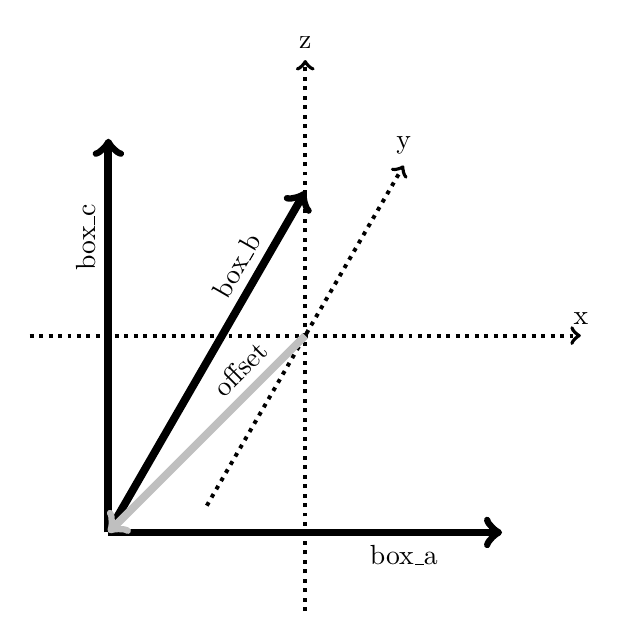
\begin{tikzpicture}
      \draw[->,black,line width=1mm] (-2.5,-2.5) -- (-2.5,2.5) node [near end,above,rotate=90] {box\_c};
      \draw[->,black,line width=1mm] (-2.5,-2.5) -- (0,1.83) node [near end,above,rotate=60] {box\_b};
      \draw[->,black,line width=1mm] (-2.5,-2.5) -- (2.5,-2.5) node [near end,below] {box\_a};

      \draw[->,black,dotted,line width=0.5mm] (-3.5,0) -- (3.5,0) node [left,above] {x};
      \draw[->,black,dotted,line width=0.5mm] (0,-3.5) -- (0,3.5) node [left,above] {z};
      \draw[->,black,dotted,line width=0.5mm] (-1.25,-2.16) -- (1.25,2.16) node [left,above] {y};

      \draw[->,lightgray,line width=1mm] (0,0) -- (-2.5,-2.5) node [near start,above,black,rotate=45] {offset};
\end{tikzpicture}
\end{center}
\caption{Scheme of system parameters describing the form and position of the simulation box}
\label{fig:interface_box_scheme}
\end{figure}

The common setup requires basic data about the simulation system. An overview can be seen in table \ref{tab:fcs_set_common_parameters}. The box vectors
describe the form of the box, in which the particles reside. For each solver there can be certain restrictions as for which kind of systems they can simulate. 
To get an idea which solvers work best (or work at all) with which systems please refer to the corresponding solver description within this documentation.
In general no solver is able to handle non-orthogonal boxes as of yet, although the interface should be able to handle these kind of boxes. The offset
enables the library to handle systems, which are shifted from the coordinate origin. For a graphical scheme, please refer to figure \ref{fig:interface_box_scheme}.
The use of periodicity is likewise restricted as the box forms. Not every solver is able to cope with every combination of periodicity. The only
common parameter not related to the system is the near field flag, which determines whether a method should perform its near field computations by itself or not.
By default, all solvers compute the interactions entirely by themselves. However, some solvers provide the possibility to delegate their near field 
computations to the main program. If the near field flag is set to false (i.e. 0), then interactions inside a solver-specific cutoff range are not computed.
The cutoff range can be retrieved (set) with a separate getter (setter) function. The solver methods provide separate potential functions for performing their
near field computations in the main program. The functionality of the near field flag is currently supported by methods P3M and P2NFFT.

\begin{table}
\begin{center}
\begin{tabular}{|p{0.2\textwidth}|p{0.45\textwidth}|p{0.25\textwidth}|}
          \hline
          parameter name        &       description                                         &   valid values                        \\
          \hline
          handle                &       pointer to parameter containing structure           &   FCS (C) or type (c\_ptr) (Fortran)   \\
          \hline
          near\_field\_flag    &       leave the near field calculations to the library    &   true ($\neq 0$) / false ($0$)       \\
          \hline
          box\_a                &       first vector describing the system box              &   $\in \mathbb{R}^3$                  \\
          \hline
          box\_b                &       second vector describing the system box             &   $\in \mathbb{R}^3$                  \\
          \hline
          box\_c                &       third vector describing the system box              &   $\in \mathbb{R}^3$                  \\
          \hline
          offset                &       offset of the lower front left corner from $\Vect{0}$&   $\in \mathbb{R}^3$                  \\
          \hline
          periodicity           &       periodicity of the system in each dimension (x,y,z) &   true / false                        \\
          \hline
          total\_particles      &       total amount of particles in the system             &   $\in \mathbb{N}^+$                  \\
          \hline 
\end{tabular}
\end{center}
\caption{Parameters for fcs\_common\_set}
\label{tab:fcs_set_common_parameters}
\end{table}

To change the solver-specific parameters, there are solver-specific setter functions. These are called \textit{fcs\_$<$solver$>$\_set\_$<$parameter$>$} where 
\textit{$<$solver$>$} is the abbreviation of the solver (table \ref{tab:solver_overview}) and parameter the name of the relevant parameter. If one wishes to change all parameters of
a solver, the use of \textit{fcs\_$<$solver$>$\_setup} is advised. A list of solver-specific parameters, that can be changed and possible values are available
in the chapters describing the solvers.

\subsection{Tuning Step}
\label{sec:tune_step}
\functiontoindex{fcs\_tune}



Most of the methods need a tuning step in which internal data structures are created according to the actual system that is simulated. Other methods
need information about the distribution of the particles within the system and between the processes. Therefore the tuning step is mandatory. In order
to tune the methods, the user has to call the function \textit{fcs\_tune} with the function call described in figure (\ref{fig:fcs_tune}). The function
calls awaits several input parameters and is similar to the function call of \textit{fcs\_run} described in the following section. First parameter of the
tuning is the handle, which was created in \textit{fcs\_init} (\ref{sec:init_step}) and then filled with \textit{fcs\_common\_set} (\ref{sec:par_setup}).
The parameter \textit{n\_locp} gives the number of particles on the local process, which is identical to the length of the array given as parameter 
\textit{charges}. For the array containing the charges, an array with thrice the length has to be supplied as parameter \textit{charges}. As final parameter,
the parameter \textit{n\_maxlocp} gives an estimation of the maximum number of particles being stored on the local process before the next call of the tuning
routine.\\
This routine is mandatory to be called, in order to grant a unified interface for the library. Some methods, e.g. PEPC, do not need this tuning step. But to be
able to switch the methods within a code without the need to greatly modify the code again, the tuning routine has to be called. If the user wants to use e.g. PEPC
as well as e.g. P2NFFT, he can use the same program (except for the method-specific setter routines), when including the tuning routine. 

\subsection{Calculation Step}
\label{sec:run_step}
\functiontoindex{fcs\_run}



The calculation step is the centerpiece of the library. Within it, the actual calculation of Coulomb interactions takes place. As mentioned in the description of tuning step,
the call to \textit{fcs\_run} (fig. \ref{fig:fcs_run}) is nearly the same, as for \textit{fcs\_tune} (see \ref{sec:tune_step}). There are two additional parameters, which are \textit{field} and
\textit{potential}. The first is the array to which the field data is added and has a size of thrice the number of local particles (\textit{n\_locp}), the latter
is the array in which the corresponding potentials are saved and has a size equal to the number of local particles (\textit{n\_locp}). All the other parameters
are equal to the parameters of \textit{fcs\_tune} (see above).


\subsection{Clean Up Step}
\label{sec:clean_up_step}
\functiontoindex{fcs\_destroy}



After the calculations are done, the memory allocated by the methods needs to be freed again. This task is done by the function \textit{fcs\_destroy} (fig. \ref{fig:fcs_destroy}).
As parameters only the FCS object is needed, in order to free memory allocated in connection with it, since the internal data structures of the methods are
administrated by those. The call to fcs\_destroy is not mandatory but the user is advised to call it, especially if he or she wants to repeat the calculation
with another method without restarting the program, since it cannot be guaranteed that more then one method can be used simultaneously without memory problems. 

\section{Error Handling}
\label{sec:error_handling}
\index{error handling}

Within the ScaFaCoS library a FCSResult type is defined. With this type return values and error messages of the methods and the interface routines are handled.
The type includes up to three pieces of information about error that have occurred during a call to a ScaFaCoS function. These pieces are a return code, an error
message and the source of the error within the library. As return values the values given in table \ref{tab:c_macros_error} can occur. In order to simplify the
error handling for the ScaFaCoS routines, the routines return \textit{NULL} as return value, instead of an allocated error object containing \textit{FCS\_SUCCESS}
as return value. The other information contained in the error type gives more information about the kind of error that occurred, e.g. if a method cannot handle
a certain system due to restrictions on periodicity, and where the error occurred within the library since the error can happen in functions called inside the
routine called by the user.\\
To get the information out of the error type, there are three functions for this task. Their calls are shown in figures \ref{fig:fcsResult_getReturnCode} to \ref{fig:fcsResult_getErrorSource}.
Due to restrictions in Fortran the message length in Fortran is capped to 256 characters.

\section{Fortran Specifics}

\begin{figure}[htb]
\begin{lstlisting}[language=Fortran,frame=trBL,breaklines,basicstyle=\small,prebreak={\raisebox{0ex}[0ex][0ex]{\ensuremath{\hookleftarrow}}}]
! Fortran
use iso_c_binding
character(kind = c_char, len = 32) :: string = "test_string"
string = trim(adjustl(string)) // c_null_char
\end{lstlisting}
\caption{Example for string truncation for strings used with ScaFaCoS}
\label{fig:example_string_fortran2c}
\end{figure}


In this section some advises are given for Fortran programmers. Since the Fortran interface is a wrapper interface above the C version of the interface trying to
stay as true to the C interface as possible, some things have to be observed. First it is advised to use the interoperable Fortran kinds delivered by the
library, which are \textit{fcs\_integer\_kind\_isoc} for integer and \textit{fcs\_real\_kind\_isoc}. With the usage of these kinds problems concerning the 
interoperability of the values is avoided. Secondly strings have to be terminated with C null characters and have to be trimmed to the correct length. An
example how this can be achieved is given in figure \ref{fig:example_string_fortran2c}. A third difference from Fortran to C is that in the Fortran interface
wherever possible the logical type is used instead of an integer value in C. This is true for every manual setter and getter connected to flags. In the parser
this exchange was not possible (see \ref{sec:interface_parser}).


\section{Further Functionality}

This sections describes some of the functionality the ScaFaCoS library has, which exceeds the pure calculation of Coulomb interactions. It also describes the
output functions within the library and the parser for parameters.

\label{sec:interface_functions}
\subsection{Near Field Solver}
\index{near field solver}
\label{sec:near_field_solver}

\todo[inline]{Should the near field solver be available to the user?}
Within the library a near field solver for given near field potentials is included. Some of the methods (P2NFFT and P3M) need to calculate separate near field
interactions, which is done by this solver. The solver uses a linked cell scheme for fast interaction calculation and uses the sorting library to create and
duplicate the particles (ghost-particles). It is able to handle periodicity and linked cell sizes that are smaller than the cut-off radius. With the near field
flag described in section \ref{sec:par_setup} the calculation of the near field portions of the Coulomb interactions can be delegated to external routines.
In order to do this the methods which support this (currently P3M and P2NFFT) provide a functions which can then be called from the user's program to calculate the
corresponding near field portions of the Coulomb interactions (see figure \ref{fig:fcs_compute_near_field} to \ref{fig:fcs_compute_near}). The aforementioned
functions are generic function that will calculate the according values for the chosen method. It is possible to check if the chosen method is able to relegate
the near field calculation by use of \textit{fcs\_method\_has\_near} (\ref{fig:fcs_method_has_near}).

\subsection{Optional Results}

It is possible to get additional results from the solver concerning the calculation. As of now the only additional result to have is the system virial. It is
possible that some solvers add additional optional results in the future. Since now only the virial is available here will be explained how to get the virial
from the solvers. For that two functions are needed, \textit{fcs\_require\_virial} (\ref{fig:fcs_require_virial}) and \textit{fcs\_get\_virial} (\ref{fig:fcs_get_virial}).
With \textit{fcs\_require\_virial} the user activates or deactivates the calculation of the virial. If set to true, the virial is activated, else it is not
calculated. If it is calculated, the user can get the calculated by the use of \textit{fcs\_get\_virial}. For that he has to pass an allocated array of nine
\textit{fcs\_float} values to the function.\\
Possibly in the next future other optional results will be implemented, if required by the community.

\subsection{Output of Interface Parameters}
\index{parameter output}
\functiontoindex{fcs\_printHandle}

For debugging purposes it is possible to print out the content of the FCS object. This is done by the use of the function \textit{fcs\_printContent} (figure \ref{fig:fcs_printHandle}).
The output shows the current values of the parameters set within the FCS object. If no changes were made to the solver-specific parameters, it shows the default
values for them. The behavior of the routine if used on a freshly created FCS object without set common parameters is undefined.

\subsection{Parser}
\index{parser}
\functiontoindex{fcs\_parser}
\label{sec:interface_parser}

To simplify the parameter input for programs basing on script file input, the ScaFaCoS library offers a parser that allows to read in parameters from a string.
The format of the passed string must adhere to the example shown in figure \ref{fig:parser_example}, while the function call can be seen in figure \ref{fig:fcs_parser}

\begin{figure}[htb]
\begin{lstlisting}[language=Fortran,frame=trBL,breaklines,basicstyle=\small,prebreak={\raisebox{0ex}[0ex][0ex]{\ensuremath{\hookleftarrow}}}]
string = "box_a,1.0,0.0,0.0,near_field_flag,1,pepc_theta,0.3"
\end{lstlisting}
\caption{Example of a parser string setting the first box vector, the near field flag and a method-specific parameter.}
\label{fig:parser_example}
\end{figure}

The format is an alteration of parameter name and value(s). In the example the first parameter to be set is a generic one, so no prefix is needed and the parameter
name is \textbf{box\_a}. Since the first box vector needs three floating point values, these are given after the parameter name, always separated by commas.
After the final parameter value, the next parameter name is expected, in the case of the example the parameter is another generic one, the \textbf{near\_field\_flag}.
Because this parameter needs only one integer value, it given and immediately followed by the next parameter name. The last parameter to be set is a solver-specific
one, the parameter \textbf{theta} from the PEPC solver. Since it is a PEPC-specific parameter, the solver name is added as a prefix, followed by the parameter name.
After it the parameter value follows, like with the generic parameters.\\
For Fortran users the advise, that every flag which is set with the parser, has to used the C syntax which requires an integer value (0 for false, 1 for true) instead
of \textit{.true.} or \textit{.false.}.

\FloatBarrier
\renewcommand\arraystretch{1.0}
